\section{Compaction as a design procedure}
\label{sec:row-3}

A long run must carry its open commitments forward and each strategy can lose one, so we turn the strategies into a compaction policy, apply it to the vending run and compare two summaries of the same history.

\subsection{A compaction policy specifies choices}
\label{sec:it-9-1}

\bi
\item \textbf{Specify:} the decisions the context must support, and the trigger.
\item \textbf{Select:} what to keep, what to summarize and what to reference.
\item \textbf{Generate:} a replacement that states facts, open items and sources.
\item \textbf{Check:} the replacement against the task, then assemble the request.
\ei

The course proposes this procedure from the objectives and mechanisms of the earlier sections. A policy specifies which future decisions the context must support and when compaction runs. It selects the material to retain verbatim, to summarize, or to leave available by reference. It generates a replacement that states facts, decisions, conditions, unresolved questions and source references explicitly. It then checks the details the task needs, inspects the resulting request and measures the total work.

Each policy choice must be evaluated, and the slide \hyperref[sec:it-10-1]{``An evaluation measures quality and total work.''} gives the checks. A token threshold can trigger compaction, and so can a task boundary or new information. The figure's trigger fires when the window fills, as in the harnesses of the strategies segment, or when the day changes, a task boundary of the vending run. Next week covers durable storage and recovery.

The four choices are the course's proposal, and no cited source proposes them. The entries are the teaching case's: the ledger line, the log, the price list and the check questions agree with the other figures.

\begin{figure}[htbp]
\centering
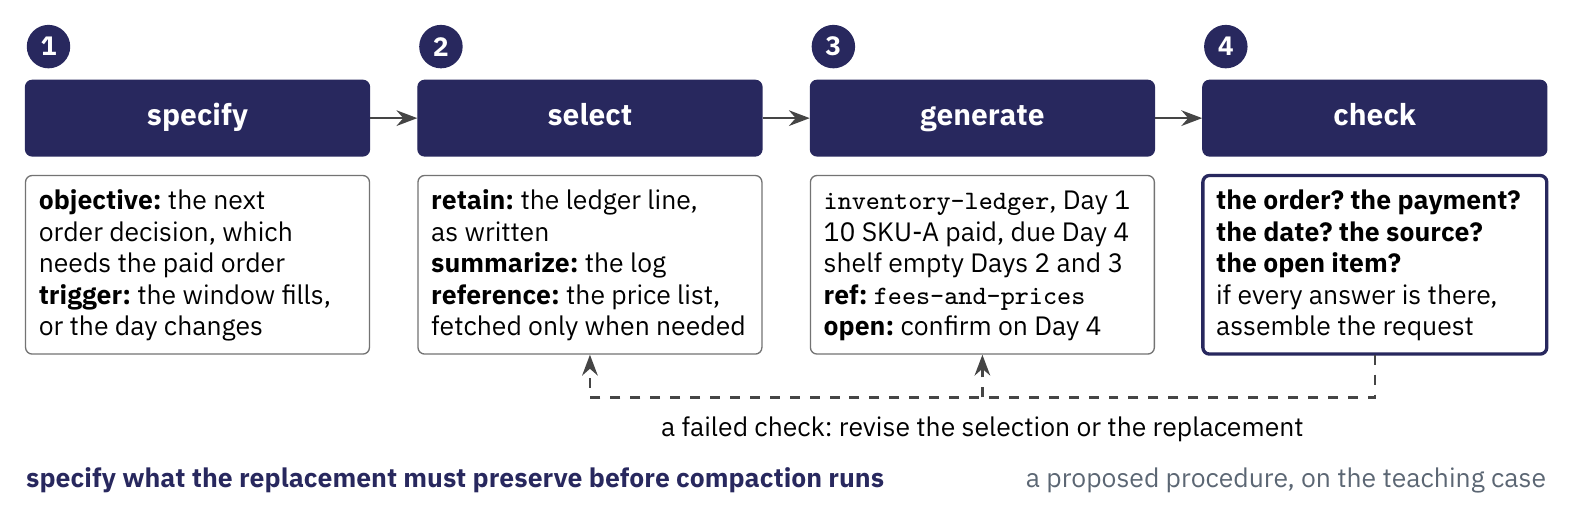
\includegraphics[width=\linewidth]{context/compaction-policy-4.png}
\caption{A compaction policy specifies choices. The figure as it stands after the build's last click.}
\label{fig:compaction-policy-4}
\end{figure}

\paragraph{The figure, stage by stage.}
\be
\item Specify: the objective is ``the next order decision, which needs the paid order'', and the trigger is ``the window fills, or the day changes'': the run compacts when the history reaches the window or when a new day begins. The grey note, ``a proposed procedure, on the teaching case'', marks the procedure as the course's own proposal.
\item Select: ``retain: the ledger line, as written'', ``summarize: the log'' and ``reference: the price list, fetched only when needed''. The ledger line keeps its exact words, the log is reduced to a summary, and the price list stays in its record until a call needs it.
\item Generate: the replacement follows from the selection. It keeps the ledger line as written with its source, ``inventory-ledger, Day 1'' and ``10 SKU-A paid, due Day 4'', summarizes the log as ``shelf empty Days 2 and 3'', points to the price list with ``ref: fees-and-prices'' and states the open item, ``open: confirm on Day 4''.
\item Check: the replacement must answer ``the order? the payment?'', ``the date? the source?'' and ``the open item?'', and the box closes with ``if every answer is there, assemble the request''. The dashed path, ``a failed check: revise the selection or the replacement'', returns to select and generate, and the navy line reads ``specify what the replacement must preserve before compaction runs''.
\ee

\begin{takeaway}A compaction policy decides what survives before any history is replaced.\end{takeaway}

\subsection{Compaction must preserve the pending order}
\label{sec:it-9-2}

\textbf{Two records describe SKU-A on Day 3 of the vending run.}

\bi
\item \textbf{Order record:} \texttt{inventory-ledger}, Day 1: 10 SKU-A paid, due Day 4.
\item \textbf{Shelf record:} \texttt{ops-log}, Days 2 and 3: the SKU-A shelf is empty, no sales.
\ei

We ask which tokens must survive to answer one question: is more SKU-A already on the way? If compaction keeps only the shelf state, the agent sees an empty shelf without the pending order. It can place a second order and pay twice. It can also conclude that the supplier failed and close the business.

This example illustrates the type of coherence failure that Vending-Bench reports. The course supplies these records as a teaching case, and we keep them beside any summary.

The records, the price and the days are illustrative, and the run is the course's teaching case.

The figure is \cref{fig:dropped-order-2} of \cref{sec:it-8-2}.

\paragraph{The figure, stage by stage.}
\be
\item The ops-log for Days 2 and 3 records ``Day 2: shelf empty, no sales'' and ``Day 3: shelf empty, no sales'', and when ``the window fills'', compaction reads the ledger and the log to ``summarize the history, drop the rest''. The navy question asks ``what must survive to answer ``is more SKU-A already on the way?''''.
\ee

\begin{takeaway}A summary must keep the paid order and its due date.\end{takeaway}

\subsection{Each summary leads to a different decision}
\label{sec:it-9-3}

\textbf{Two summaries of the same history reach Day 4.}

\bi
\item \textbf{Summary A} drops the paid order, so the agent orders again and pays twice.
\item \textbf{Summary B} keeps the order, its due date and its source, so the agent waits.
\ei

Both summaries illustrate the teaching case. Summary A reads ``SKU-A is out of stock.'' It loses the paid order and its expected arrival, so the agent places a second order or closes the business. Summary B reads ``SKU-A shelf-empty Days 2 and 3. Ordered 10 units on Day 1 (paid), expected Day 4. Sources: inventory-ledger Day 1 and ops-log Days 2 and 3. Pending: confirm delivery on Day 4.'' The figure shortens it to the order, its source and the check. B keeps the paid order, the expected date and the route to the source.

B is longer because the decision needs the open order. Its references help only while the ledger stays available. A causes the failure of the previous section, and B avoids it.

The two summaries and the second order are the course's illustration.

\begin{figure}[htbp]
\centering
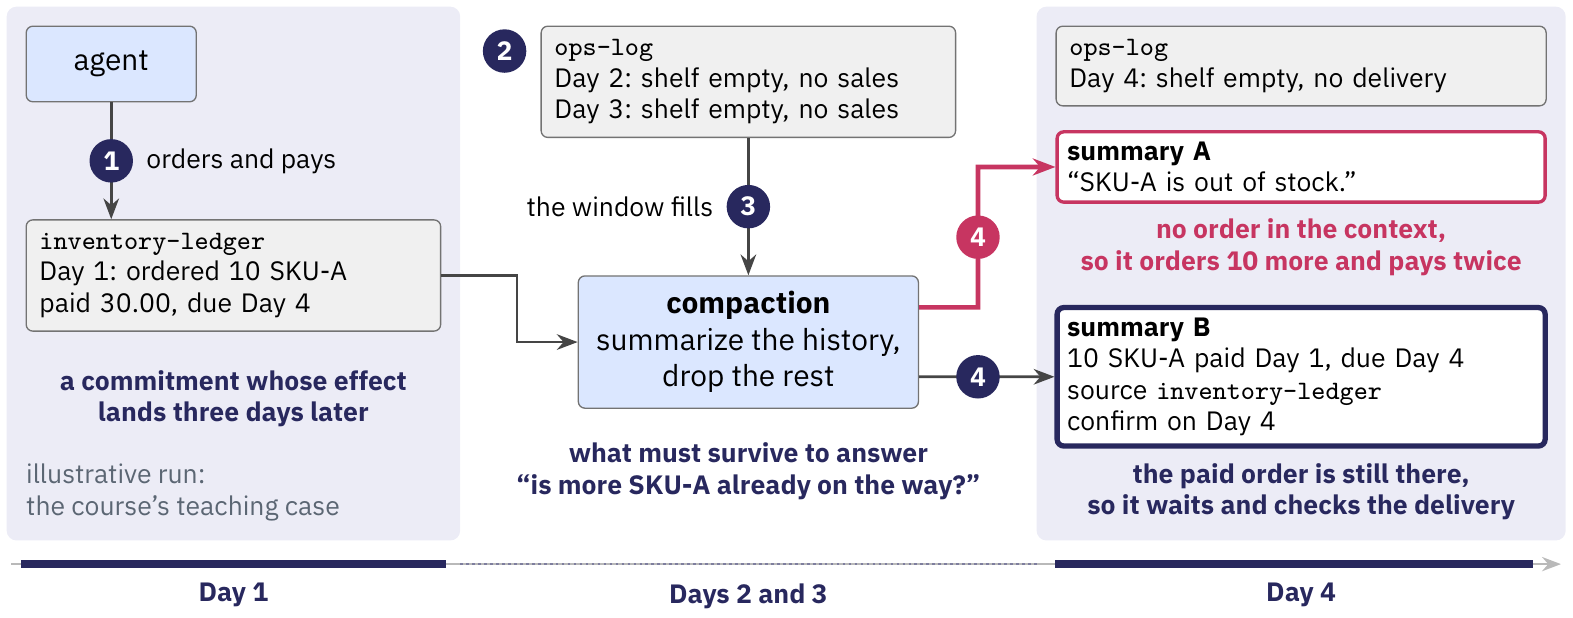
\includegraphics[width=\linewidth]{context/dropped-order-4.png}
\caption{Each summary leads to a different decision. The figure as it stands after the build's last click.}
\label{fig:dropped-order-4}
\end{figure}

\paragraph{The figure, stage by stage.}
\be
\item The ops-log for Days 2 and 3 records ``Day 2: shelf empty, no sales'' and ``Day 3: shelf empty, no sales'', and when ``the window fills'', compaction reads the ledger and the log to ``summarize the history, drop the rest''. The navy question asks ``what must survive to answer ``is more SKU-A already on the way?''''.
\item Summary A reaches Day 4 along the magenta path of event 4 and says only ``SKU-A is out of stock.'' The ledger line is gone from the context, and the new ops-log line ``Day 4: shelf empty, no delivery'' mentions no order, so the magenta verdict reads ``no order in the context, so it orders 10 more and pays twice''.
\item Summary B is the other outcome of the same compaction step, numbered 4 again in navy, and keeps ``10 SKU-A paid Day 1, due Day 4'', ``source inventory-ledger'' and ``confirm on Day 4''. Summary A settles to a magenta outline, and the navy verdict reads ``the paid order is still there, so it waits and checks the delivery''.
\ee

\begin{takeaway}A replacement is judged against the decision it must support.\end{takeaway}

\subsection*{Key points}
\bi
\item A compaction policy decides what survives before any history is replaced.
\item A summary must keep the paid order and its due date.
\item A replacement is judged against the decision it must support.
\ei
